\hypertarget{background}{%
\section{Background}\label{background}}

The transition towards a future low-carbon economy is driven globally by
the Paris Agreement {[}Pari15{]}, which recognises the need for
sustainable development worldwide to counter the threats of climate
change. The European Union (EU) is committed to reduce greenhouse gas
(GHG) emissions by 2050 to 80-90 \% below 1990 levels {[}Ener12{]}. As
the energy industry is responsible for the highest share of
anthropogenic GHG emissions, importance is placed on how changes in
energy systems can help achieve these GHG emission reduction targets
{[}Ener12{]}.

A number of opportunities exist for the decarbonisation of the energy
industry. The International Renewable Energy Agency (IRENA), in their
renewable energy roadmap study, has identified renewable energy as
having the highest potential in reducing energy-related carbon dioxide
(CO2) emissions globally, which is closely followed by energy efficiency
and electrification with renewable energy {[}Glob18{]}. In a 2018
political agreement, the EU member states agreed upon a target of at
least 32 \% of the demand being met with renewables by 2030, through
national targets of the individual member states {[}ReneND{]}. The
electricity demand in the transport sector is also expected to increase
due to expected petrol and diesel engine bans and subsequently the
electrification of road transport {[}Worl17{]}.

The energy system is also transitioning towards a decentralised system
with more consumer participation and new forms of flexibilities,
including sector coupling, demand-side management (DSM), energy
conversion and storage, cross-border interconnection and curtailment.
This allows demand patterns to shift to better suit the generation
patterns in systems with high penetration of variable renewable energy
(VRE) resources, such as solar and wind {[}Lund17{]}, {[}Towa18{]}.
However, this requires cooperation involving many actors with various
responsibilities and dependencies that interact within this energy
system, and opens up the opportunity to perform interdisciplinary
research work in the area of energy system analysis.

The ENSYSTRA - ENergy SYStems in TRAnsition Innovative Training Network
has been established to address the challenges of the energy transition
with interdisciplinary collaboration and regional cooperation involving
academia, government and industry {[}AbouND{]}. ENSYSTRA is centred on
the North Sea region and focusses on performing interdisciplinary
modelling work involving technology, economics, social science and
humanities, and combining various modelling approaches in different
levels and resolutions. ENSYSTRA aims to keep an open science approach,
which will allow the resulting models to be subject to full scientific
scrutiny.

Energy systems models, which are tools used to project the future energy
supply of a country or region {[}Herb12{]}, is the centre of ENSYSTRA.
The figure below explains the energy systems modelling process using a
system analysis approach {[}Kroo15{]}. This process starts with creating
a model of the actual energy system by simplifying and conceptualising
the present system. This conceptualised system with all assumptions is
then mathematically solved to produce numerical results. These results
can then be interpreted and conclusions can be drawn regarding the
future energy system. Such conclusions form the evidence-base for
decision makers, resulting in policy implications or operational
strategies that help achieve these climate targets.

\begin{figure}
\centering
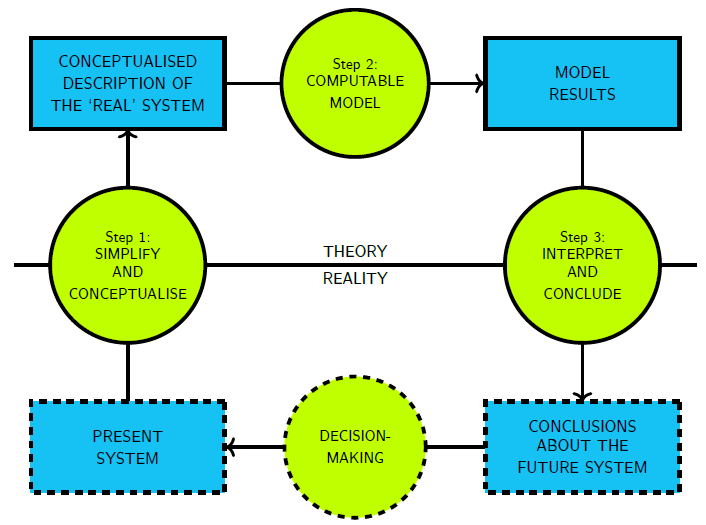
\includegraphics{images/system-analysis.png}
\caption{The system analysis approach applied on the energy system
modelling process, adapted from Krook-Riekkola 2015 {[}Kroo15{]}.}
\end{figure}

There are 15 early-stage researchers (ESRs) across four work packages
(WPs) in ENSYSTRA, as shown in the figure below. The research project
entitled ``Development of a real-time optimisation solution for
dispatchable energy supply units'' is conducted by ESR 9, who is
enrolled as a PhD student at University of Stavanger (UiS) in Norway.
This project is within WP 2 (technology prospects and development
pathways), which focusses on technological options for the energy
transition, mainly in terms of techno-economic performance over time.
For this research project, the technology focus is on the digitalisation
of the electricity sector. As the electricity system transitions into
smart systems, the system will have an increasing amount of sensors and
controllers that continuously record measurements of the system
{[}Lund17{]}. Advancements in these technologies mean that data that is
fast, heterogeneous and high in volume from the electricity system will
be generated. Data with these characteristics must be managed and
analysed effectively to gain insights on the electricity system, which
can then be converted to strategies that optimise the system
{[}Mana12{]}. This project will specifically investigate how artificial
intelligence (AI) can play a role in the transition to a low-carbon
electricity system by utilising high resolution data of the system. The
next section will investigate this, as well as explain what is meant by
``real-time'' and ``dispatchable'' in the context of electricity systems
in this project.

\begin{figure}
\centering
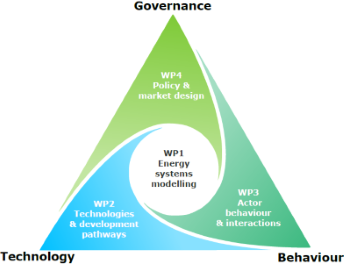
\includegraphics{images/wp.png}
\caption{Interactions between the four WPs of the ENSYSTRA project.
Source: ENSYSTRA {[}AbouND{]}.}
\end{figure}
